\documentclass[aspectratio=169]{beamer}
\usepackage{babel}
% \usepackage[german]{babel}

\usepackage{tikz, transparent, colortbl, pgfplots}
\usepackage[export]{adjustbox}
\usepackage[skins,theorems]{tcolorbox}
 
\usetikzlibrary{automata,positioning}
\setbeamercovered{transparent}
\pgfplotsset{compat=1.18}
\tcbset{highlight math style={enhanced,colframe=red,colback=white,arc=0pt,boxrule=1pt}}

% Useful Read:
% https://www.overleaf.com/learn/latex/Beamer

\title{Molecular Dynamics}
\subtitle{Group A}
\author{Haoyuan Ma \and Zhengying Zhao \and Anatoly Weinstein}
\date{31st of October 2025}

\newcommand{\framebackground}[2]{
    \begin{tikzpicture}
        \transparent{#1}
        \node[inner sep=0] at (current page.center) {
            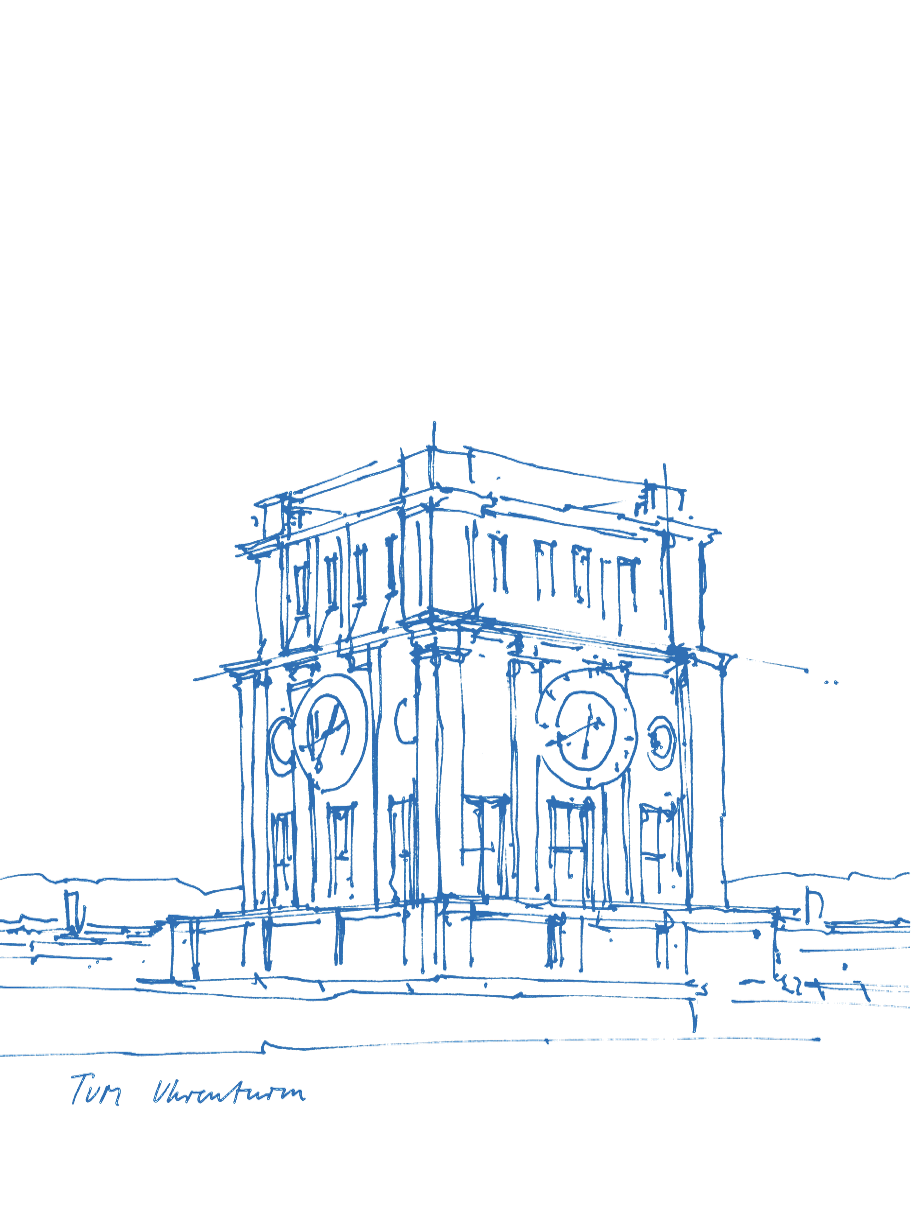
\includegraphics[height=\paperheight, right]{./media/tum-uhrenturm.png}
        };
        \transparent{1}
        \node[anchor=south, text width=\paperwidth, text height=1.5cm, draw=none, align=center] at (current page.south) {
            \insertpagenumber
        };
        \transparent{#2}
        \node[anchor=south, text width=\paperwidth, text height=1.5cm, draw=none, align=right] at (current page.south) {
            \small Haoyuan Ma, Zhengying Z, Anatoly W. \,\,
        };
    \end{tikzpicture}
}

\newcommand{\headerframe}{
    \usebackgroundtemplate{
        \framebackground{0.2}{1}
    }
}

\newcommand{\simpleframe}{
    \usebackgroundtemplate{
        \framebackground{0}{1}
    }
}

\newcommand{\blue}[1]{{\color{beamer@blendedblue} #1}}
\newcommand{\yellow}[1]{{\color[HTML]{AF8F10} #1}}
\newcommand{\gray}[1]{{\color[HTML]{8F8F8F} #1}}
\newcommand{\red}[1]{{\color[HTML]{FF5F5F} #1}}

\begin{document}

%
% Frame
%
\usebackgroundtemplate{\framebackground{0.2}{0}}
\begin{frame}
    \maketitle
\end{frame}

\simpleframe\begin{frame}{The test run of the simulation}
    \begin{figure}
        \centering
        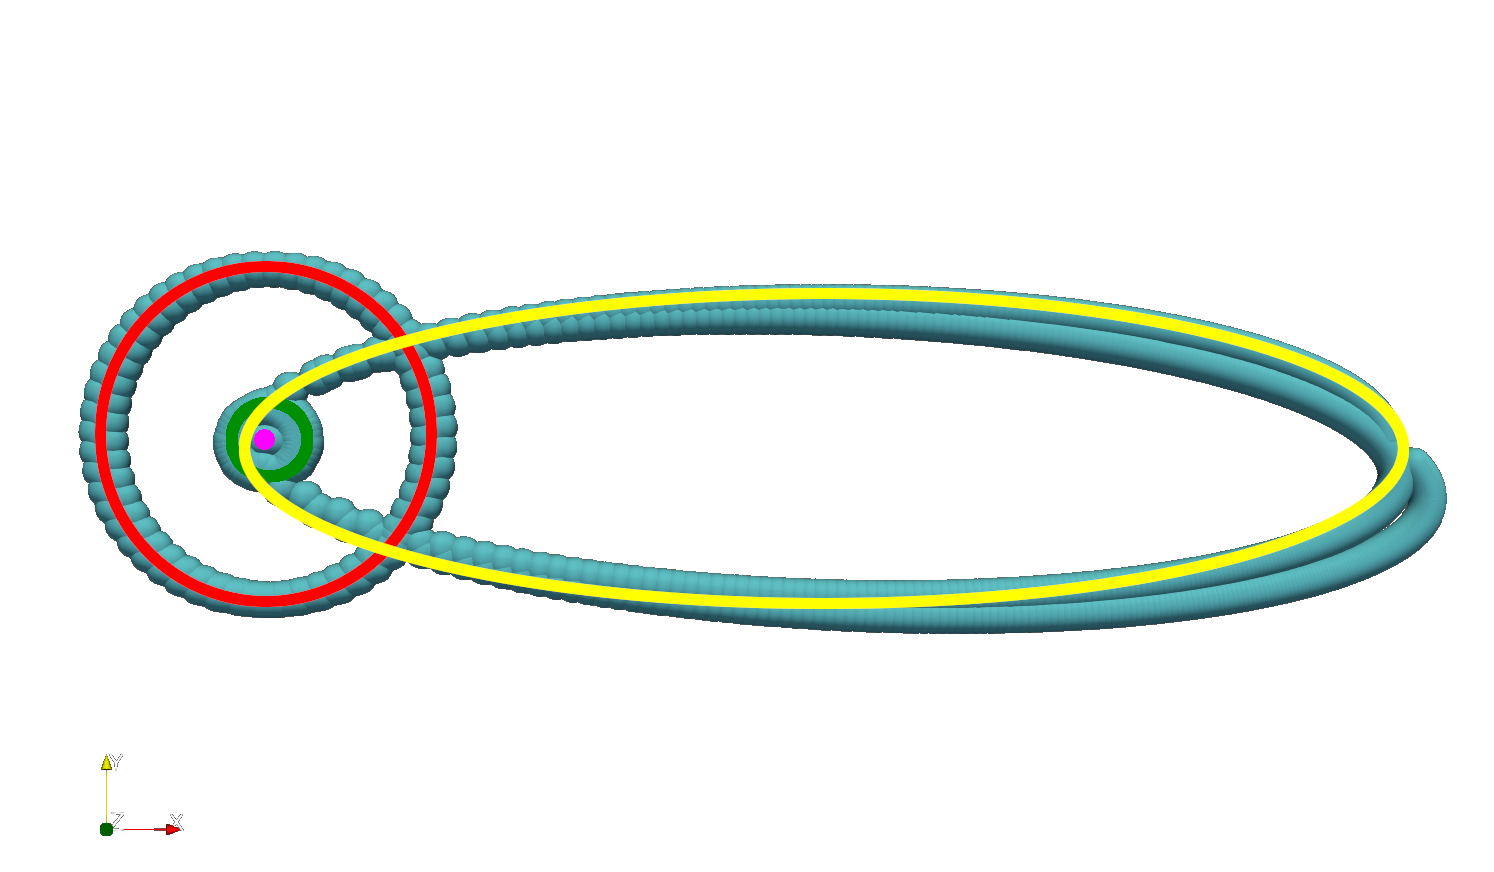
\includegraphics[width=0.6\textwidth]{media/t1000_d0.14_annotated.png}

        \par\vspace{4pt}
        \begin{center}
            {\color[HTML]{FF00FF}$\bullet$}~Earth \qquad
            {\color[HTML]{008F00}$\bullet$}~ISS \qquad
            {\color[HTML]{FF0000}$\bullet$}~Moon \qquad
            {\color[HTML]{8F8F00}$\bullet$}~Halley's Comet
        \end{center}
    \end{figure}
\end{frame}

\simpleframe\begin{frame}{Comparing $\Delta t$ in Simulations}
    \begin{columns}
        \begin{column}{0.5\textwidth}
            \begin{figure}
                \centering
                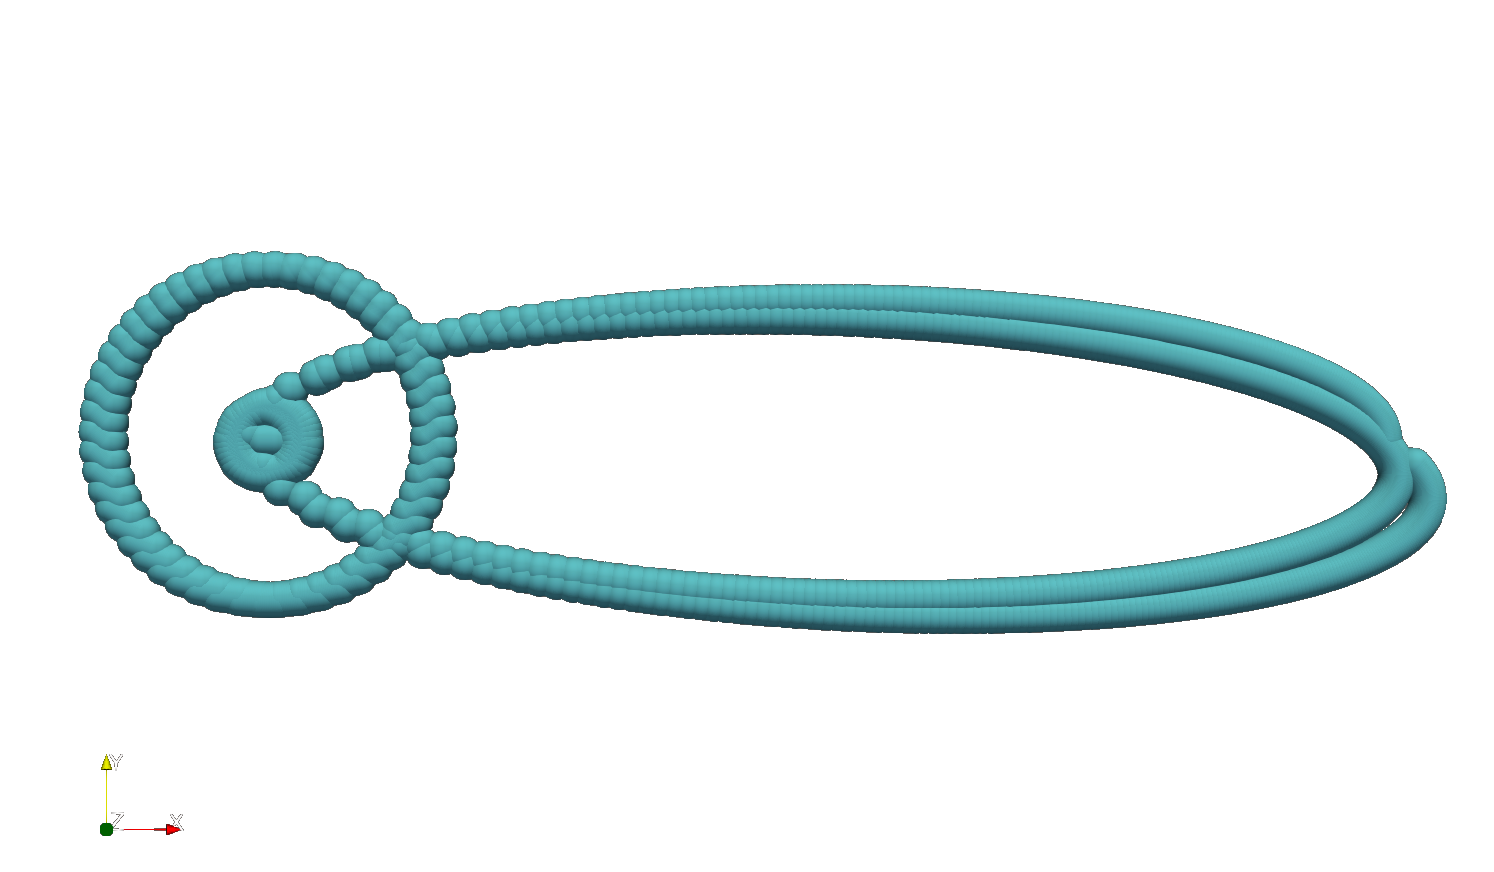
\includegraphics[width=0.6\textwidth]{media/t1000_d0.14.png}
                \caption{Simulation with $\Delta t = 0.14$}
            \end{figure}
        \end{column}
        \begin{column}{0.5\textwidth}
            \begin{figure}
                \centering
                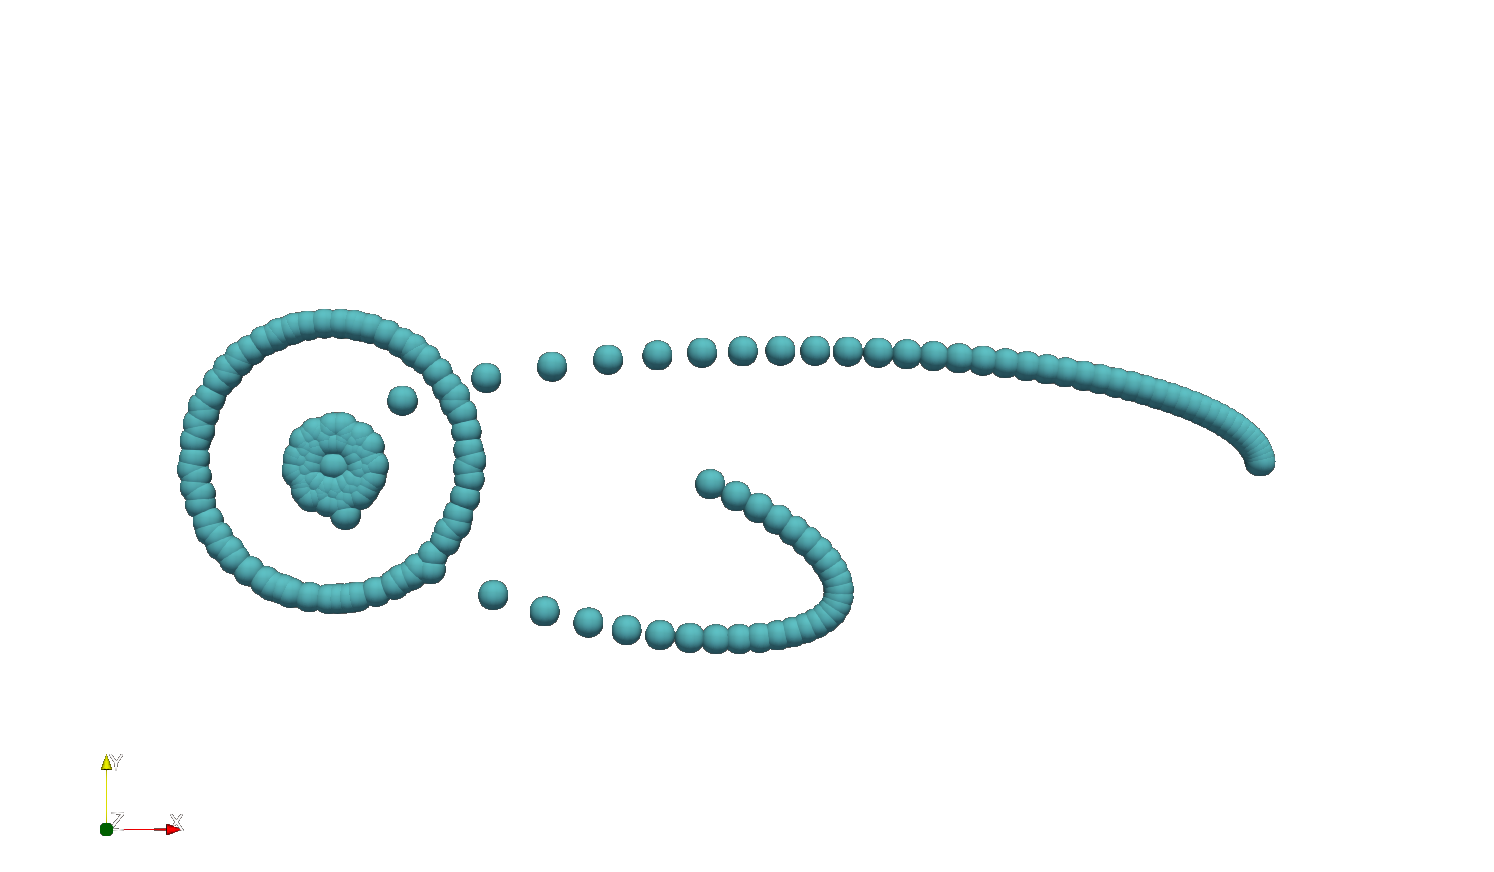
\includegraphics[width=0.6\textwidth]{media/t400_d0.56.png}
                \caption{Simulation with $\Delta t = 0.56$}
            \end{figure}
        \end{column}
    \end{columns}
    
    \begin{figure}
        \centering
        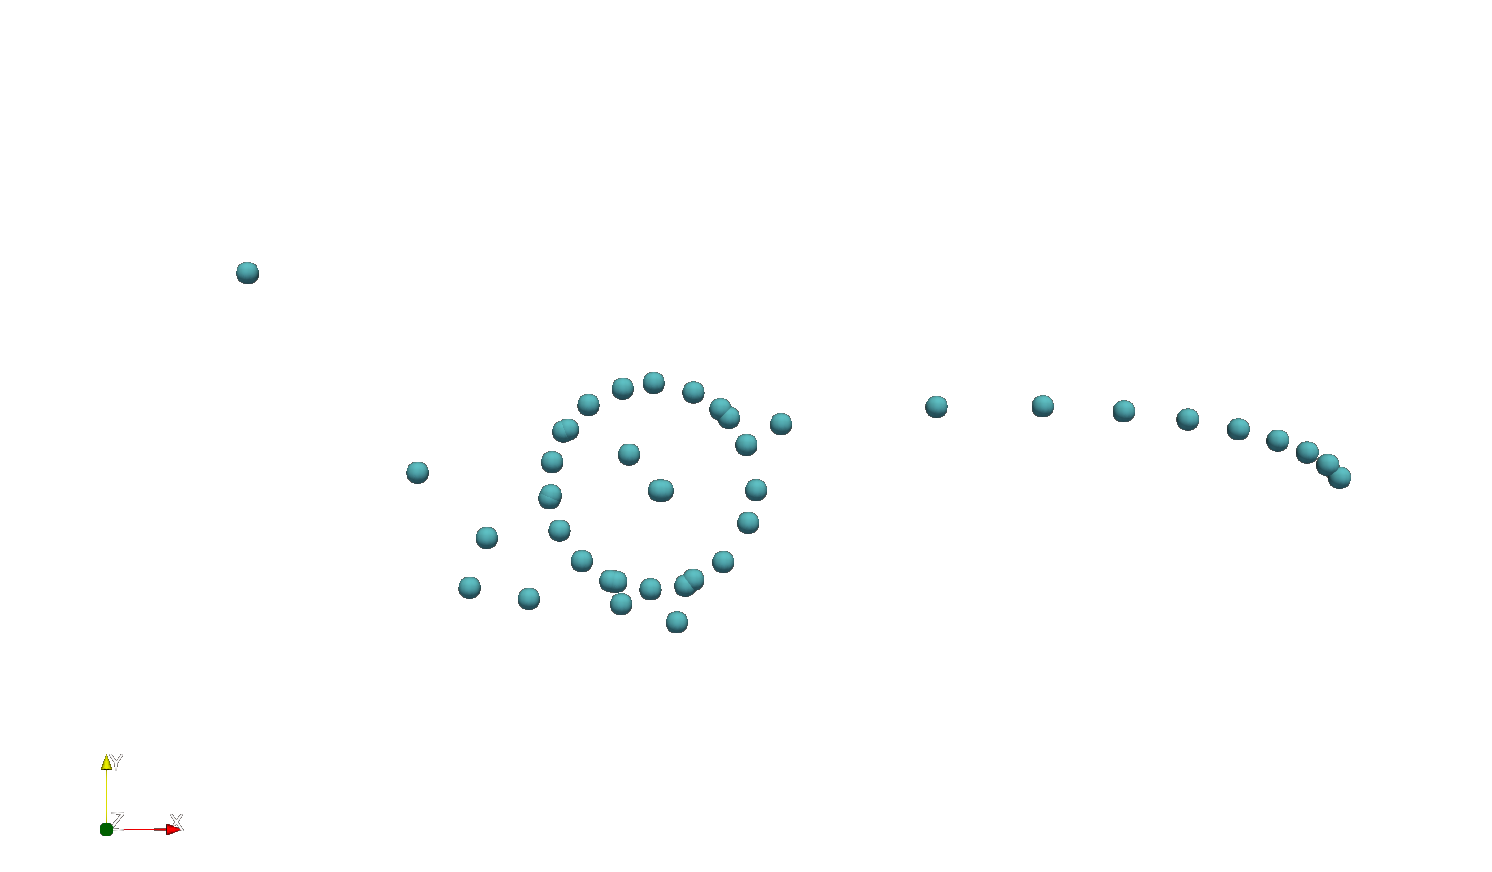
\includegraphics[width=0.3\textwidth]{media/t500_d2.24.png}
        \caption{Simulation with $\Delta t = 2.24$}
    \end{figure}

    \vspace{0.5cm}

    Conclusion: \red{Results deviate for different $\Delta t$!}

    Leads to the question: \blue{How to choose an appropriate $\Delta t$?}
\end{frame}

\simpleframe\begin{frame}{Comparing $\Delta t$ in Simulations}
    \begin{columns}
        \begin{column}{0.3\textwidth}
            \centering
            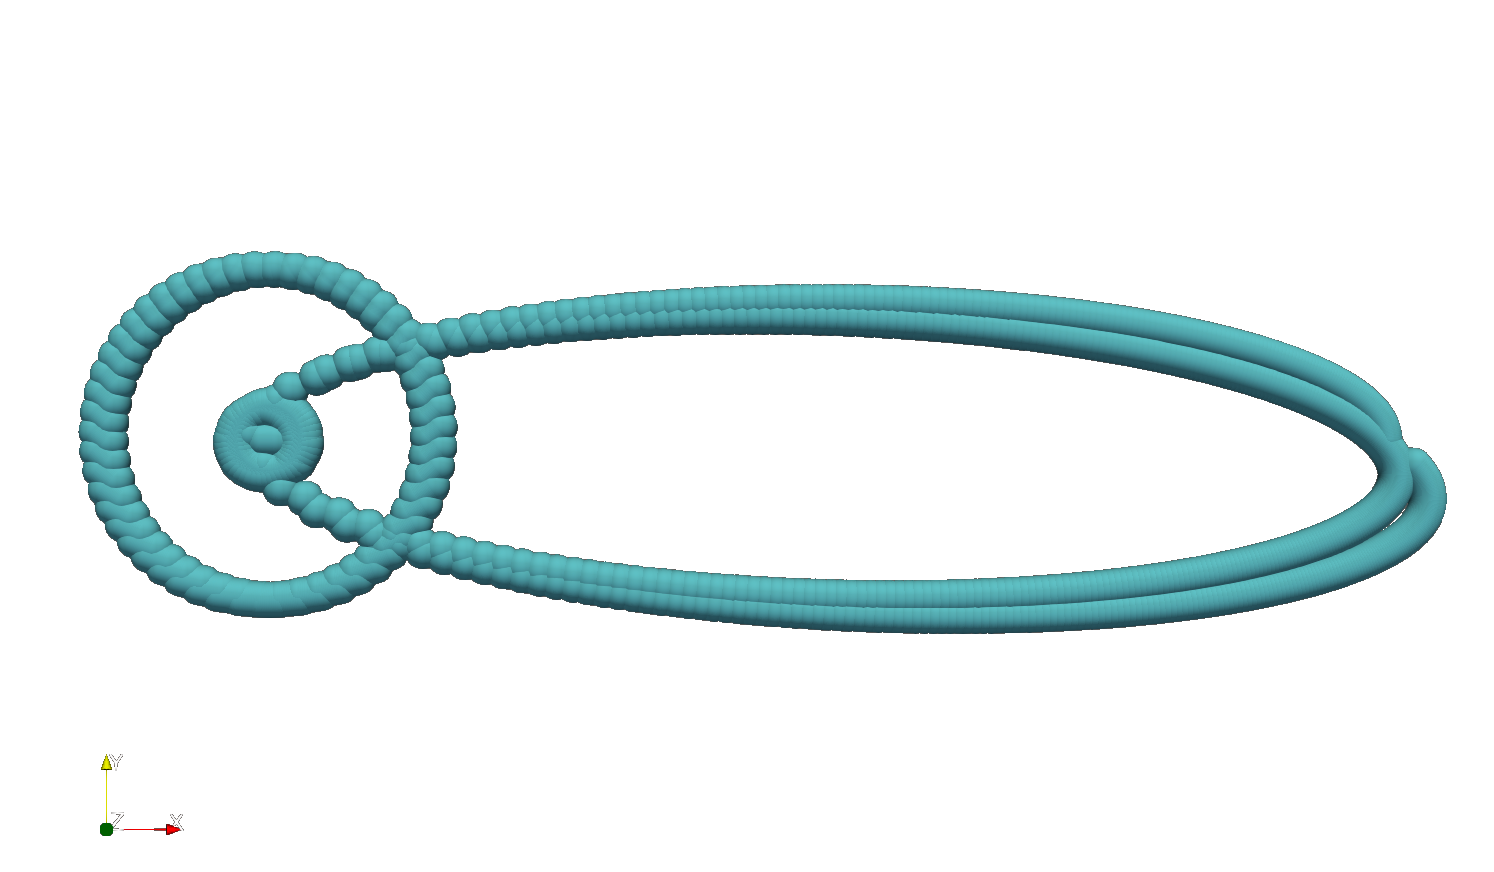
\includegraphics[width=0.9\textwidth]{media/t1000_d0.14.png}
        \end{column}
        \begin{column}{0.3\textwidth}
            \centering
            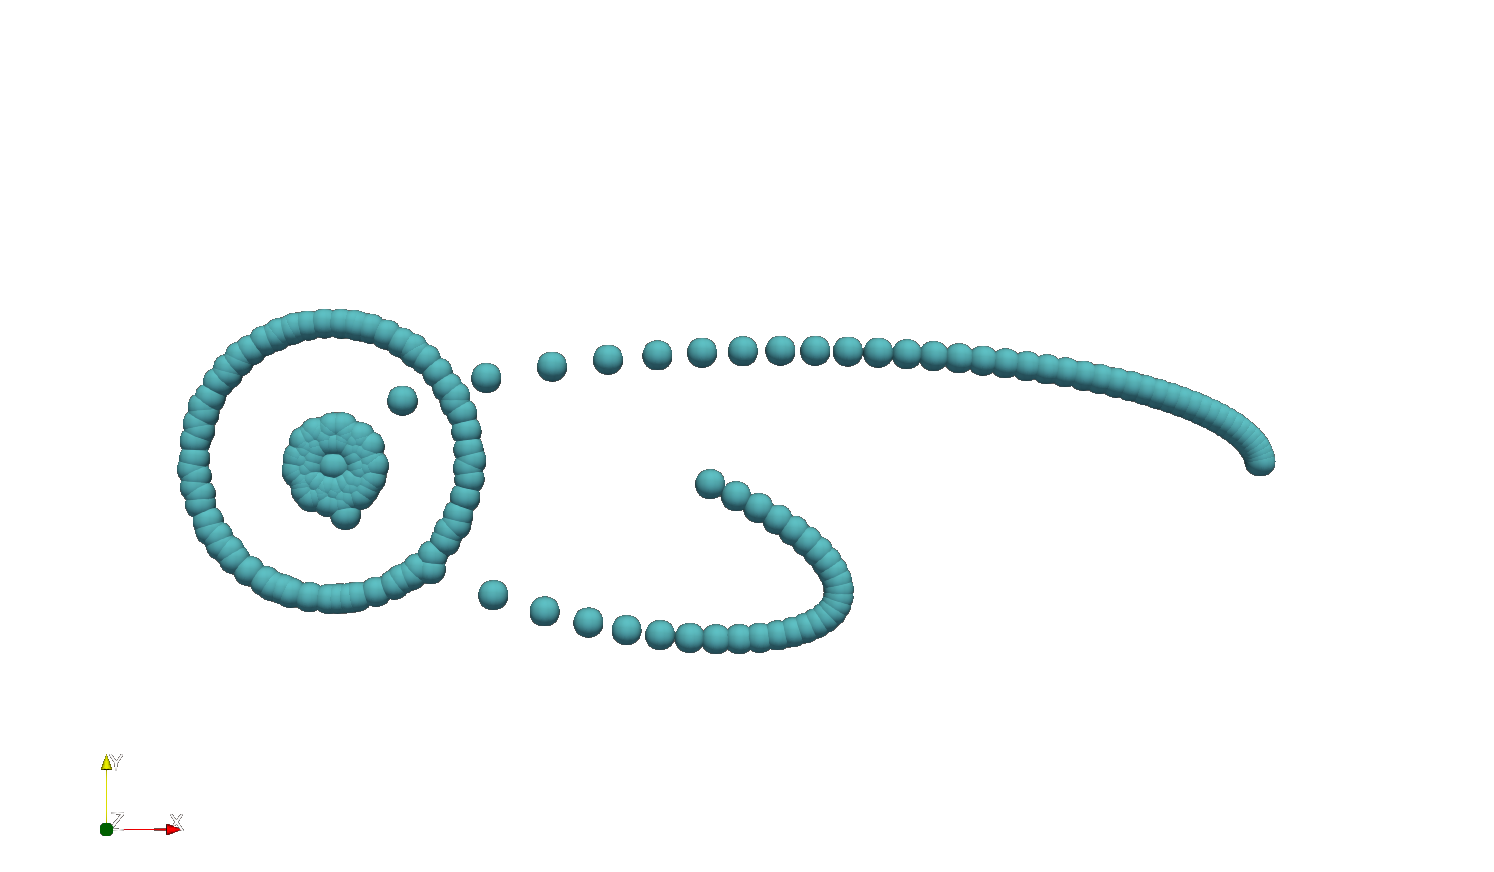
\includegraphics[width=0.9\textwidth]{media/t400_d0.56.png}
        \end{column}
        \begin{column}{0.3\textwidth}
            \centering
            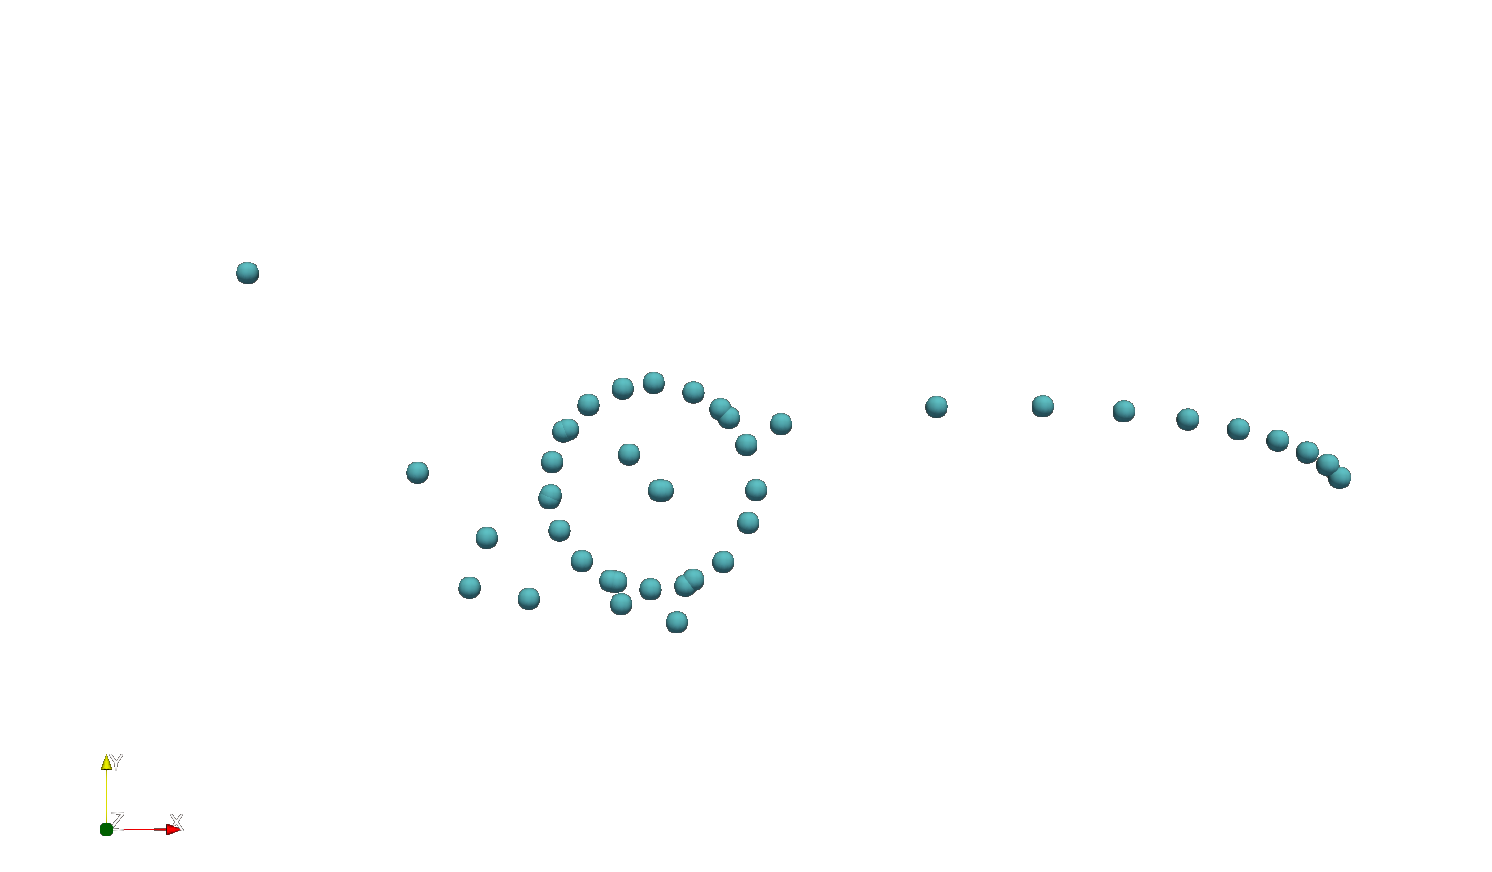
\includegraphics[width=0.9\textwidth]{media/t500_d2.24.png}
        \end{column}
    \end{columns}

    \vspace{0.5cm}
    Conclusion: \red{Results deviate for different $\Delta t$!}

    Follow-up question: \blue{How to choose an appropriate $\Delta t$?}
\end{frame}

\headerframe\begin{frame}{That's it – for now, at least}
    \begin{center}
        \LARGE\blue{Thank you for your attention!}
    \end{center}
\end{frame}

\end{document}
